\section{Related Work}\label{sec:existing_work_appendix}

\begin{figure*}[!ht]
	\centering
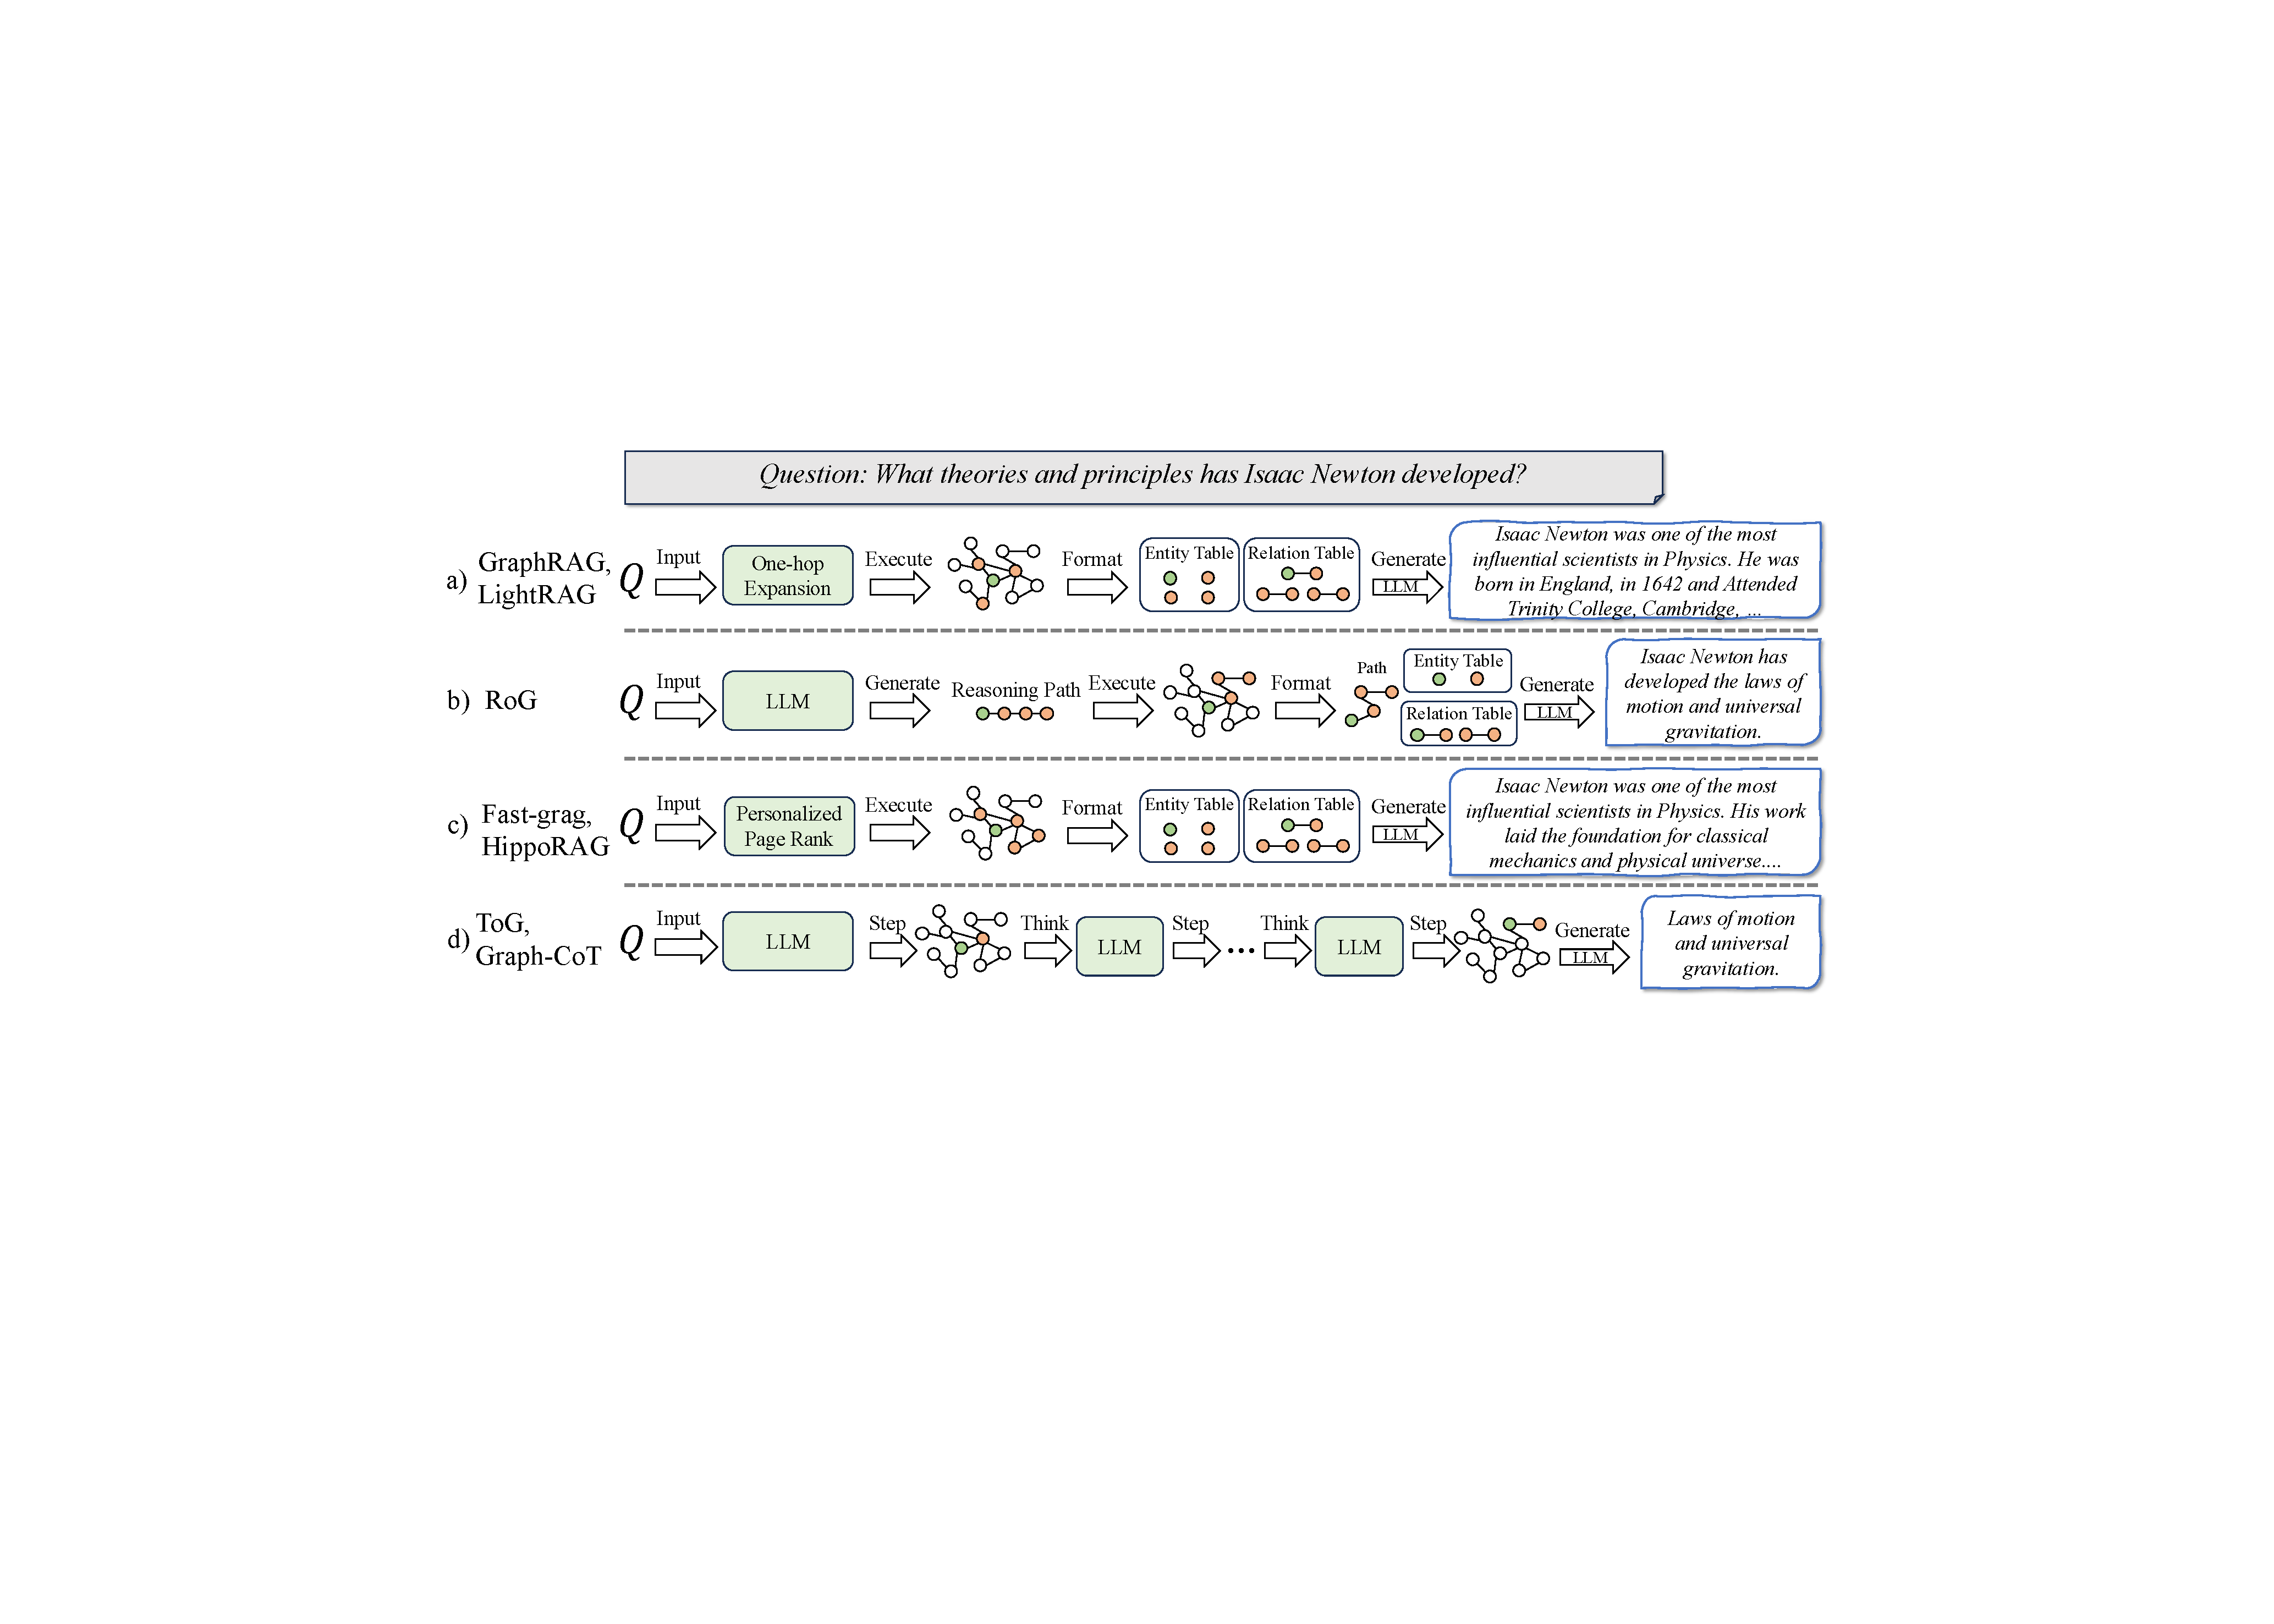
\includegraphics[width=\textwidth]{figures/existing_work.pdf}
	% \vspace{-4mm}
	\caption{Workflow demonstration and comparison of existing GraphRAG methods.}
	\label{fig:existing_work}
	 % \vspace{-2mm}
\end{figure*}

Many GraphRAG approaches are proposed to tackle KGQA tasks or answer general user questions about the knowledge graph, and they differ in the adopted graph traversal methods. In the following, we introduce representative GraphRAG methods and \autoref{fig:existing_work} illustrates the workflow of them.

As shown in \autoref{fig:existing_work}a, GraphRAG~\cite{ms_graphrag} and LightRAG~\cite{lightrag} use one-hop neighbor expansion to retrieve neighboring entities and relations of the anchor entities (entities that appear in the question), and return two tables as the retrieved context to the LLM as external grounding knowledge. While one-hop neighbor expansion is efficient in execution, this method fails to capture long-distance knowledge and thus cannot well answer questions that require reasoning paths beyond one-hop.

RoG~\cite{rog}, as depicted in \autoref{fig:existing_work}b, prompts the LLM to generate faithful reasoning paths that can be followed on the knowledge graph and returns the retrieved paths for generation. Faithful reasoning paths directly point from the anchor entity to the answer entities without involving useless noise in the context. However, it is only applicable when the question itself explicitly reveals concrete relation constraints. If the question is abstract in its predicate chain, e.g., asking about general information of an entity or relationships with another entity, no faithful reasoning paths could be given.

The workflow of Fast-graphrag~\cite{fast_graphrag} and HippoRAG~\cite{hipporag} is shown in \autoref{fig:existing_work}c. It retrieves entities and relations by running the well-studied random walk method, Personalized PageRank, and returns those with a relevance score greater than a threshold. Due to the diversity and complexity of graph questions, this fuzzing relevance matching that purely depends on the structure of knowledge graph might not accurately find what the question exactly requires.

The workflow of ToG~\cite{tog} and Graph-CoT~\cite{graphcot} is displayed in \autoref{fig:existing_work}d. They hand over the decision on every step of graph traversal to the LLM, prompting it with the current neighbors and all previous contexts to determine which neighbors to explore next. Traversal stops when the LLM thinks it reaches the answer, and then the answer entities are returned as results. This chain-of-thought manner is adaptable to various cases by leveraging the reasoning adaptability in LLMs. However, they end up at high cost in both response latency and token usage, which is expensive to use in real applications.